\documentclass[12pt]{extreport}
\usepackage{cmap} 
\usepackage[T2A]{fontenc} % Поддержка русских букв
\usepackage[utf8]{inputenc} % Кодировка utf8
\usepackage[english,russian]{babel} % Языки: русский, английский
\usepackage{fontspec}
\setmainfont{Times New Roman}

\usepackage{listings}
\usepackage{graphicx}
\usepackage{amsmath,amsfonts,amssymb,amsthm,mathtools} 
\usepackage{pgfplots}
\usepackage{filecontents}
\usepackage{float}
\usepackage{indentfirst}
\usepackage{eucal}
\usepackage{enumitem}
\frenchspacing

\usepackage{indentfirst} % Красная строка

\usetikzlibrary{datavisualization}
\usetikzlibrary{datavisualization.formats.functions}

\usepackage{amsmath}


% Для листинга кода:
\lstdefinestyle{asm}{
	language={[x86masm]Assembler},
	backgroundcolor=\color{white},
	basicstyle=\small\sffamily,
	keywordstyle=\color{blue},
	stringstyle=\color{red},
	commentstyle=\color{gray},
	numbers=left,
	numberstyle=\tiny,
	stepnumber=1,
	numbersep=5pt,
	frame=single,
	tabsize=4,
	captionpos=b,
	breaklines=true
}

\usepackage[left=3cm,right=2cm, top=2cm,bottom=2cm,bindingoffset=0cm]{geometry}
% Для измененных титулов глав:
\usepackage{titlesec, blindtext, color} % подключаем нужные пакеты
\definecolor{gray75}{gray}{0.75} % определяем цвет
\newcommand{\hsp}{\hspace{12pt}} % длина линии в 20pt
% titleformat определяет стиль
\titleformat{\chapter}[hang]{\Huge\bfseries}{\thechapter\hsp\textcolor{gray75}\hsp}{0pt}{\Huge\bfseries}


% plot
\usepackage{pgfplots}
\usepackage{filecontents}
\usetikzlibrary{datavisualization}
\usetikzlibrary{datavisualization.formats.functions}

\begin{document}
%\def\chaptername{} % убирает "Глава"
\thispagestyle{empty}
\begin{titlepage}
	\noindent \begin{minipage}{0.15\textwidth}
	
\includegraphics[width=\linewidth]{./inc/img/b_logo.jpg} 
	\end{minipage}
	\noindent\begin{minipage}{0.9\textwidth}\centering
		\textbf{Министерство науки и высшего образования Российской Федерации}\\
		\textbf{Федеральное государственное бюджетное образовательное учреждение высшего образования}\\
		\textbf{~~~«Московский государственный технический университет имени Н.Э.~Баумана}\\
		\textbf{(национальный исследовательский университет)»}\\
		\textbf{(МГТУ им. Н.Э.~Баумана)}
	\end{minipage}
	
	\noindent\rule{18cm}{3pt}
	\newline\newline
	\noindent ФАКУЛЬТЕТ $\underline{\text{«Информатика и системы управления»}}$ \newline\newline
	\noindent КАФЕДРА $\underline{\text{«Программное обеспечение ЭВМ и информационные технологии»}}$\newline\newline\newline\newline\newline
	
	\begin{center}
		\noindent\begin{minipage}{1.3\textwidth}\centering
			\Large\textbf{  Отчет по лабораторной работе №1}\newline
			\textbf{по дисциплине "Операционные системы"}\newline
			\textbf{по теме "Дизассемблирование INT 8h"}\newline\newline
		\end{minipage}
	\end{center}
	
	\noindent\textbf{Студент} $\underline{\text{Миронов Г.А.~~~~~~~~~~~~~~~~~~~~~~~~~~~~~~~~~~~~~~}}$\newline\newline
	\noindent\textbf{Группа} $\underline{\text{ИУ7-53Б~~~~~~~~~~~~~~~~~~~~~~~~~~~~~~~~~~~~~~~~~~~~~~}}$\newline\newline
	\noindent\textbf{Оценка (баллы)} $\underline{\text{~~~~~~~~~~~~~~~~~~~~~~~~~~~~~~~~~~~~~~~~~~~~~}}$\newline\newline
	\noindent\textbf{Преподаватели} $\underline{\text{Рязанова Н.Ю.~~~~~~~~~~~~~~~~~~~~~~~~~~}}$\newline\newline\newline
	
	\bgroup 
	\centering
		\vfill
		
		Москва
		
		\the\year
		~г.

	\egroup 
\end{titlepage}

\chapter{Полученный дизассемблированный код}

\section{Листинг INT8h} 

\begin{lstinputlisting}[
	caption={Листинг INT 8h},
	label={lst:int8},
	style={asm}
]{./inc/asm/win95_1.lst}
\end{lstinputlisting}

\section{Листинг процедуры sub\_1}

\begin{lstinputlisting}[
	caption={Листинг процедуры sub\_1},
	label={lst:sub_1},
	style={asm}
]{./inc/asm/win95_2.lst}
\end{lstinputlisting}

\chapter{Схема алгоритмов}

\section{Схема алгоритма обработчика INT8h}

\begin{center}
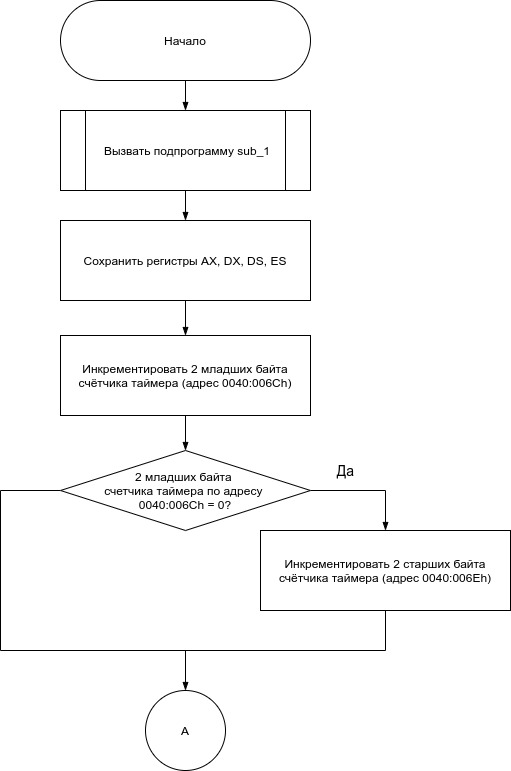
\includegraphics[scale=0.6]{./inc/img/int8h_1.jpg} 
\newpage
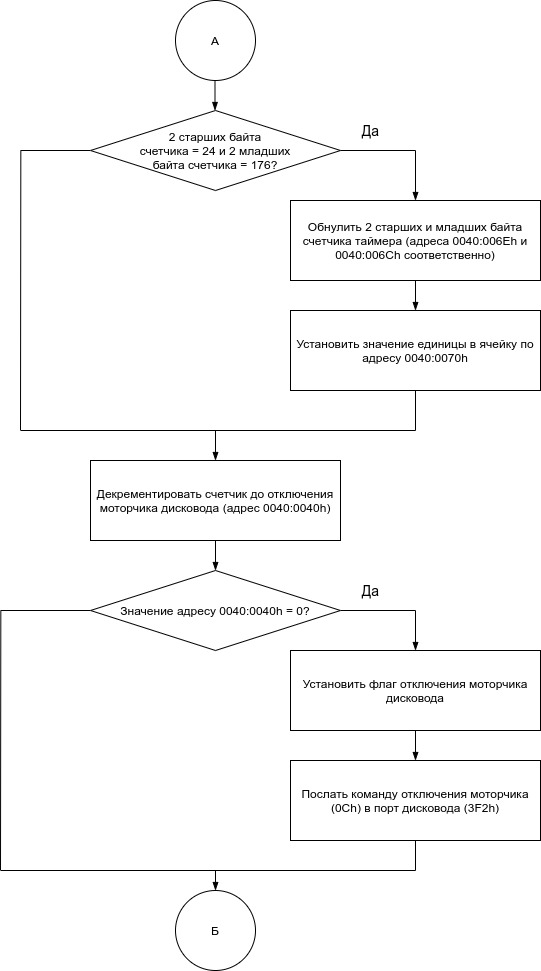
\includegraphics[scale=0.6]{./inc/img/int8h_2.jpg} 
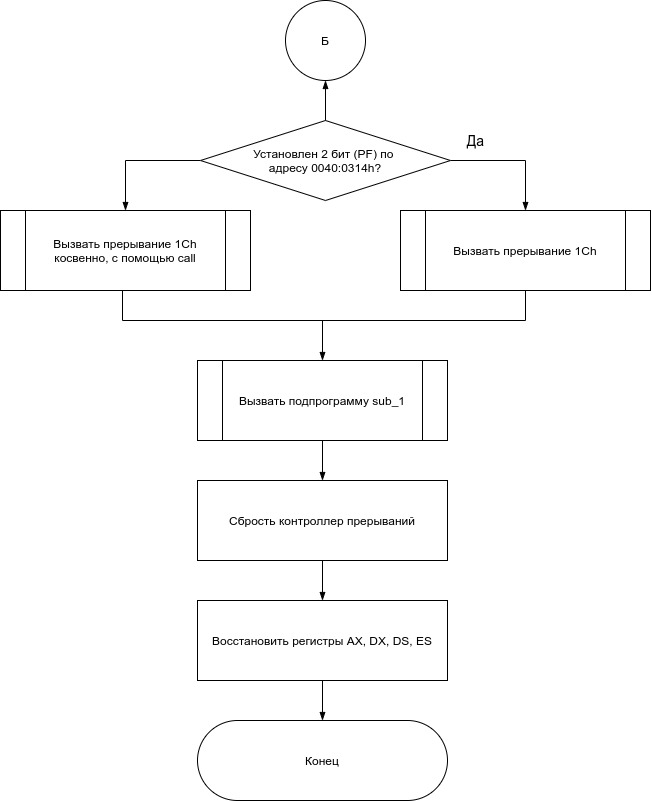
\includegraphics[scale=0.6]{./inc/img/int8h_3.jpg} 
\end{center}

\clearpage
\subsection{Схема алгоритма процедуры sub\_1}

\begin{center}
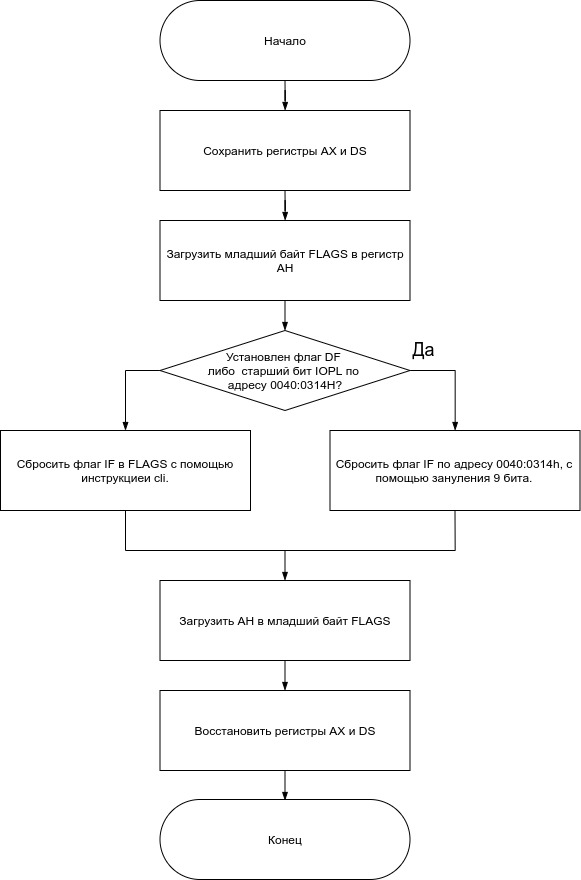
\includegraphics[scale=0.7]{./inc/img/sub_1.jpg} 
\end{center}

\end{document}